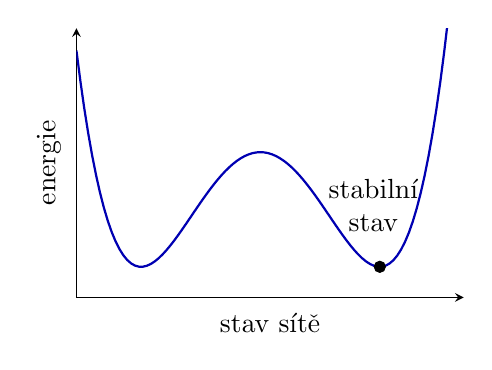
\begin{tikzpicture}
    \begin{axis}[
        width=6.5cm,
        height=5cm,
        xmin=0, xmax=6,
        ymin=0, ymax=2.2,
        axis lines=left,
        xlabel={stav sítě},
        ylabel={energie},
        xlabel near ticks,
        ylabel near ticks,
        xtick=\empty,
        ytick=\empty,
        samples=100,
        domain=0:6
    ]
        \addplot[thick, blue!70!black]
            {0.08*(x-1)^2*(x-4.7)^2+0.25};

        \addplot[only marks, mark=*]
            coordinates {(4.7,0.25)};

        \node[align=center]
            at (axis cs:4.6,0.75)
            {stabilní\\stav};
    \end{axis}
\end{tikzpicture}
